\chapter{Microcontrolador}
{\color{red} Puedes dedicar un capítulo a
analizar los frameworks de ML para empotrados, para acabar
determinando que vas a escoger TinyML, justificando por qué los
escoges y por qué descartas los demás, otro capítulo para
determinar qué microcontrolador vas a escoger y por qué, analizando
varias alternativas comparando las ventajas e inconvenientes de cada
una de ellas y justificando por qué escoges finalmente Arduino, y en
general, un capítulo por cada decisión importante de tecnología que
hayas hecho.}
\section{Planificación}
\subsection{Elección del microcontrolador}
Como ya se especificó en la sección \textit{(\ref{reqHW})Requisitos hardware}
necesitamos ciertas características inmutables. Para poder quedarnos con un
microcontrolador, antes debemos hacer el ejercicio de búsqueda de algunos
candidatos y analizar sus características. La búsqueda se ha sustentado
en encontrar dispositivos compatibles con \textit{TensorFlow Lite}.
\begin{itemize}
    \itemsep0em 
    \item SparkFun Edge
    \item Arduino Nano Sense 33 BLE
    \item STM32F746G
    \item Adafruit EdgeBadge
    \item STM32
    \item ESP32
\end{itemize}
La \textit{ESP32} al igual que la \textit{STM32} pueden descartarse debido a que
carecen de sensores relacionados
con el movimiento, se les podrían integrar periféricamente, pero sería algo
más molesta su inserción en una carcasa. Y dado que tenemos alternativas que
cuentan con estos sensores, podemos permitirnos descartarlas.

Por otro lado la \textit{Adafruit EdgeBadge} es una placa muy llamativa,
potente y llena de posibilidades, pero cuenta con unas dimensiones superiores
a lo que se busca.

Respecto a la \textit{STM32F746G} el inconveniente es la bajísima disponibilidad
y los plazos de envío desorbitados. Por tanto tampoco podemos contar con ella.

Por lo que la disyuntiva se plantea entre la \textit{Arduino Nano Sense 33 BLE}
y la \textit{SparkFun Edge}. {\color{green}La realidad es que en este punto
compré ambas porque los tiempos de entrega no eran muy esperanzadores, de hecho
compré varias Nano y una Sparkfun para ponerme a trabajar cuanto antes.
No sé si debería ser franco con esto o decir que elegí la Nano, que en realidad
acabé eligiendo porque cuenta con proyectos en los que me he podido
apoyar. En definitiva, no sé si decir lo que ocurrió tal cual o ir directamente
al motivo por el que acabé usando la Nano, que es lo que hay provisionalmente}.
En este caso la decisión no está motivada por características técnicas, que
además son muy parecidas en ambos dispositivos, sino que una de ellas ofrece
algo fundamental cuando se trabaja por primera vez en un campo y más aún
cuando se cuenta con limitación de tiempo.
El motivo taxativo es la documentación que provee Arduino, así como el apoyo
de su activa comunidad y el gran volumen de proyectos que podemos consultar y
que hacen uso de esta misma placa. Sumado a que este microcontrolador es
prácticamente el más extendido para \textit{Machine Learning}, por tanto
no solo encontraremos multitud de sketches en los que apoyarnos, sino que
muchos de ellos o la práctica mayoría estarán enfocados al \textit{Machine
Learning}. El mayor valor añadido con el que puede contar un dispositivo
que se empleará partiendo de pocos conocimientos y con restricción temporal.

De su propia nomenclatura podemos extraer todos los elementos precisados para
este proyecto:
\begin{itemize}
    \itemsep0em 
    \item Arduino: Garantiza que encontraremos documentación, y asistencia
    y proyectos de otros usuarios.
    \item Nano: Posee unas dimensiones convenientes para poder incorporarlo
    en un lápiz.
    \item Sense: Cuenta con diversos sensores, concretamente con una \textit{IMU}
    que provee de \textit{giroscopio} y \textit{acelerómetro}.
    \item BLE: Bluetooth de bajo consumo que proporcionará autonomía
    y libertad de movimiento.
\end{itemize}

\subsection{Elección de las tecnologías}
El entorno de desarrollo escogido será el propio \textit{Arduino IDE}, debido
a que nos facilita mucho el trabajo en ciertas tareas como el acceso al puerto
serie, la instalación de librerías para Arduino y sus dispositivos, o la carga
del sketch en la placa con un solo click. Adicionalmente, se hará uso de
\textit{Visual Studio Code} en los periodos de programación sin interacción
con el microcontrolador, dado que es un entorno más cómodo para gestionar
varios archivos simultáneamente y programar durante sesiones algo más largas.

Por otro lado, se hará uso de \textit{TensorFlow Lite} por múltiples razones
como que es de código abierto, gratuito, se complementa a la perfección con
muchas otras herramientas de alto nivel(entre otras, \textit{Keras} o \textit{Scikit Learn}),
etc. Pero al igual que en las elecciones anteriores, lo que más decanta la balanza
es siempre la expansión y utilización frente a sus alternativas. Ya que esto se
traduce en, generalmente, mayor documentación, mayor interacción de la comunidad,
más proyectos que poder consultar y más experiencias de otros usuarios que pueden
ser de interés.


\section{Diseño}
\subsection{Estructura del sketch}
El sketch se distribuirá en diferentes secciones, la principal,
\textit{deep\_pen.ino}(extensión propia de \textit{Arduino}, empleada en
el archivo principal de sus sketchs) incluirá todo lo relativo a la
configuración previa de las características del microcontrolador y las
habituales funciones \textit{setup()} y \textit{loop()}.

En \textit{deep\_pen\_model\_data} encontraremos exclusivamente el modelo
de la red neuronal entrenado y listo para funcionar en formato binario,
dada la carencia de sistema de archivos.

\textit{labels} será la sección que ocupe la gestión de las etiquetas del
modelo; definición y traducción etiqueta a letra.

El apartado \textit{rasterize\_stroke} rasterizará el movimiento recogido,
transformándolo en las imágenes que sirven como entrada para el modelo.

Por último, \textit{stroke\_collector} estará reservado a la recolección
del movimiento y la configuración del servicio \textit{BLE} vinculado
a la recolección de muestras para el modelo.
\newpage

\subsection{Servicio BLE}
Pese a que se implementarán dos servicios, uno de ellos es parte del \textit{Data collector},
sección extraida del proyecto de \textit{Pete Warden}\textsuperscript{\cite{petewardenmw}}
y por tanto no la desarrollaré más allá de una breve explicación en su apéndice.
Se describirá, por tanto, solamente el servicio implementado de cero:
\textit{letterSenderService}.

Previo a la descripción del diseño, debemos entender cómo funciona esta versión
bluetooth de bajo consumo.

\begin{teoria}{Configuración \textit{BLE}(Bluetooth Low Energy)\textsuperscript{\cite{BLEAndroid, BLEguide, BLEOreilly}}}
    \color{mitexto}
    El funcionamiento de este bluetooth de bajo consumo es notoriamente
    disidente de la versión general, tanto que tenemos que hablar de una
    estructura propia y que será clave para poder hacer uso de esta
    herramienta.
    Esta estructura jerárquica está definida por \textbf{\textit{Atributos}}
    {\footnotesize(Attributes)}.
    Cada uno de los elementos a continuación enumerados son
    \textbf{\textit{Atributos}}, todos ellos identificados por un
    \textbf{\textit{UUID}}{\footnotesize(Universally Unique Identifer)}:
        \begin{enumerate}
            \itemsep0em 
            \item \textbf{\textit{Servicios}} {\footnotesize(Services)}\\
            {\small Agrupaciones de características. Un servicio suele
            componerse de características vinculadas al ámbito del servicio.
            Generalmente cada servicio corresponde a una prestación del
            dispositivo}
            \item \textbf{\textit{Características}} {\footnotesize(Characteristics)}\\
            {\small Cada característica contiene un tipo(\textbf{\textit{UUID}})
            de característica, sus propias propiedades y sus
            propios permisos. Y continuando con
            la disposición jerárquica, cada característica está formada
            por ninguno, uno o múltiples descriptores.\\
            Representan estados del dispositivo, datos de la configuración
            del mismo o simplemente un dato correspondiente a alguna
            función del servicio.}
            \item \textbf{\textit{Descriptores}} {\footnotesize(Descriptors)}
            {\small La unidad mínima de la estructura. Es la que contiene
            la información transmitida por cada comportamiento de una
            característica y sus metadatos asociados.}
        \end{enumerate}
    \end{teoria}


El servicio (\textit{letterSenderService}) está compuesto por dos características:
rx(\textit{rxChar}) y tx(\textit{txChar}). Tomaremos estas características
como canales de comunicación unidireccionales. Han sido denominados teniendo
en cuenta la placa como
sistema de referencia; \textit{rx} será la característica receptora de datos y 
\textit{tx} la característica transmisora.\newline
Utilizaremos el canal \textit{tx} para transmitir la letra y el canal \textit{rx}
a modo de gestor de flujo; para la comunicación con el programa de usuario. Cuando
el interfaz de usuario reciba la letra y la almacene, escribirá en el canal
\textit{rx} la correspondiente señal para que el canal \textit{tx} se borre
y pueda dar paso a una nueva letra.

\begin{figure}[h]
    \centering
    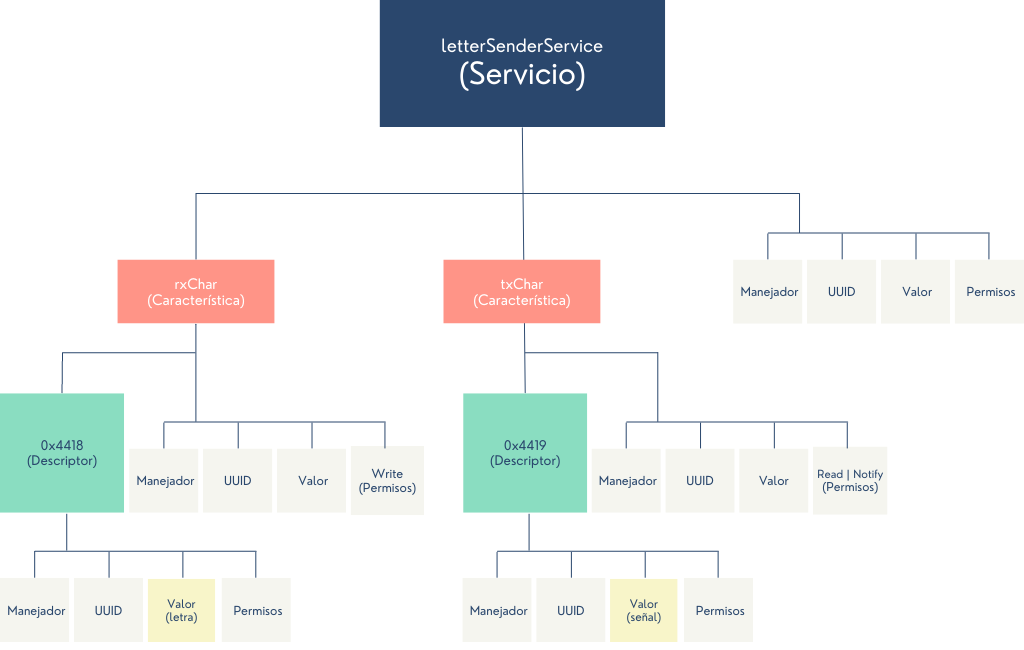
\includegraphics[width=1\textwidth]{capturas/BleLetterSenderService.png}\\[-0,40cm]
    \caption{Esquema de la estructura planteada para el servicio \textit{BLE}}
\end{figure}

\section{Implementación}
{\color{red} Después tendrías que explicar el diseño completo, es decir, cómo
encajan todas las piezas (incluyendo el PC de desarrollo) para poder
desarrollar el sistema. Recuerda que diseñar es explicar qué hace
cada cosa, qué datos envía, qué recibe, etc., pero no cómo. El
cómo se hace cada cosa es ya desarrollo.}\\~\\
{\color{red}Después podrías hablar del desarrollo, de qué cosas concretas hay
que hacer, configurar el IDE de Arduino, hacer sketchs, generar los
datos de entrenamiento, entrenar la red, convertirla para el
microcontrolador, etc., pero sin entrar en los detalles técnicos (que
estarán en los apéndices correspondientes). Este capítulo sería
como una guía que te vaya diciendo cómo ir consultando los
apéndices y qué es lo importante en cada apéndice para que el que
quiera pueda replicar tu proyecto. Pero debe estar escrito para que
que no quiera replicar el proyecto se entere bien de qué cosas has
hecho, de su dificultad, de lo que has tenido que aprender para poder
hacer el desarrollo, etc. El tribunal tiene que entender la
envergadura de lo que has hecho, qué cosas has hecho cómo de
difíciles han sido, etc. Eso es vital. Por eso sacamos todos los
detalles técnicos a los apéndices, para que se puedan centrar en lo
que les quieres contar. Los apéndices son sólo para demostrar que de
verdad lo has hecho, pero lo importante es el rollo que cuentas acerca
de cómo ha sido el desarrollo. Espero que hayas cogido la idea.}
\subsection{Configuración BLE \textsuperscript{\cite{ladvien}}}
En el primer bloque del sketch, encontramos la configuración de
la placa respecto a \textit{BLE}(Bluetooth Low Energy).

La configuración de permisos de las características son consecuentes con
su cometido. La característica de lectura, tendrá permisos de escritura
para que la \textbf{central} pueda escribir los valores que la placa leerá.
Análogamente la característica de escritura tendrá permisos de lectura y
notificación.


\begin{teoria}{Roles de las partes en conexiones bluetooth\textsuperscript{\cite{BLEOreilly}}}
    \color{mitexto}
    Al darse una conexión bluetooth, existen ciertas implicaciones inherentes
    a la propia conexión. Y es que siempre habrá una de las partes que
    se lucra de los servicios de la(s) otra(s).\\
    Pues bien, los dispositivos que se gestionan o se benefician de los
    servicios de otros, se conocen como \textbf{central} y los que proveen,
    son los \textbf{periféricos}.
\end{teoria}
El resultado de la configuración del servicio \textit{BLE} obedece completamente
al diseño planteado.

Finalmente se deben definir una serie de manejadores para gestionar los
distintos eventos relacionados con el servicio \textit{BLE} tales como
conexiones y desconexiones o recibo de señal por el canal de lectura
\textit{rx}.


\subsection{Función 'setup()'\textsuperscript{\cite{andriyadimw,petewardenmw}}}
En esta sección, como de constumbre, se hará el ajuste propio para la
la ejecución de nuestro sketch.\newline
Es reseñable mencionar que la placa con la que estamos trabajando solo
posee la memoria flash y SRAM características de los dispositivos de estas
prestaciones. Sin embargo tenemos que almacenar alguna información
imprescindible, como lo es el propio binario del modelo de nuestra
red neuronal; la reserva de algunas secciones de memoria también tendrán
que ser gestionadas.\newline
El modo de afrontar estas limitaciones será trabajar con la propia flash
del dispositivo a modo de región de almacenamiento, creando arrays en la
propia flash que harán las veces de mecanismo de almacenamiento. Esto
supone solventar la carencia de almacenamiento de una forma eficiente,
ya que el coste de acceso a la informción será mínimo, sin lecturas
externas.\newline
Esto se repetirá en varias circunstancias del sketch, por ejemplo,
en este bloque de setup, será necesario reservar un área para las labores
de E/S y memoria intermedia de las acciones con tensor.

\begin{lstlisting}[firstnumber=62,title=Fragmento de \textit{deep\_pen.ino}]
    /************************ SETUP FUNCTION ************************/
    // Setting the area of memory reserved to tensor input-output actions.
    constexpr int TensorAreaSize = 30 * 1024;
    uint8_t tensor_arena[TensorAreaSize];
\end{lstlisting}

Y más adelante se hará uso de la misma técnica para almacenar el binario de
nuestro modelo, entre otros.

\subsubsection{BLE e IMU setup}
En esta primera etapa de setup, se fijarán los parámetros para la configuración
de la placa; en primer lugar, se dará para la \textbf{IMU}(\textit{Inertial
Measurement Unit}) y el \textbf{BLE}.
\begin{teoria}{Por qué es necesario configurar la \textbf{IMU}\textsuperscript{\cite{imuteoria}}}
    La \textbf{IMU} es una parte fundamental de este proyecto, ya que es
    el dispositivo contenido en la placa que gestiona las mediciones de
    aceleración y velocidad del movimiento y que consta para ello de
    acelerómetro y giroscopio.
\end{teoria}

\begin{problemas}{Librería Arduino\_LSM9DS1}
    \color{mitexto}
    Uno de los problemas con esta parte del código, fue que
    la librería \textit{Arduino\_LSM9DS1}\textsuperscript{\cite{lsm9ds1}} necesaria para poder trabajar con
    la \textbf{IMU}, tiene varias versiones.
    Al haber leído para algunos de los proyectos TFLite de
    arduino, que era recomendable utilizar su primera versión, fue la elegida.
    Sin embargo esta primera versión, no posee una de las funciones
    necesarias para trabajar con la \textbf{IMU} en nuestro caso,
    que es el llenado
    contínuo de la FIFO de lectura de medidas recogidas, que por defecto
    funciona en \textit{oneShotMode}, es decir, llenado a ráfagas.
    Es necesario poder disponer de la función para trabajar en tiempo
    real con la predicción de letras y también es imprescindible para la
    recolección de muestras, como se verá más adelante.\\
    Por lo que la solución es o bien añadir manualmente la función en la
    librería, o bien actualizarla a la versión \textit{1.1.0}.
\end{problemas}

Por lo que solo resta fijar los parámetros creados para \textbf{BLE},
vincular sus señales con manejadores de los eventos y hacer lo propio
con la \textbf{IMU}.\\
Cabe destacar que adicional a la configuración \textbf{BLE} descrita, también
se incorpora otro servicio con la característica \textit{strokeCharacteristic},
menos interesante de explicar, ya que utilizaré el método de recolección de
muestras de \textit{Pete Warden} para uno de los ejemplos
\textit{TFLite de Arduino}: \textit{magic\_wand}\textsuperscript{\cite{petewardenmw}}.

\subsubsection{Setup de nuestro modelo}
Parte de máxima trascendencia, ya que, es imprescindible configurar de
manera adecuada los parámetros del modelo para que el reconocimiento
se de manera óptima.\\
Una vez obtenemos el modelo definido en \textit{deep\_pen\_model\_data.cpp}.

Se deben establecer las micro-operaciones que se darán en el modelo
para tener definido el repertorio en tiempo de ejecución que utilizará
nuestro interprete.\textsuperscript{\cite{intro-tensor-micro}}
Como alternativa más cómoda, pero a costa de un mayor uso de memoria,
del cual no podemos abusar dada la naturaleza de nuestro dispositivo;
es plausible usar \textit{tflite::AllOpsResolver}, que cargará todas las
operaciones disponibles para \textit{TFLite}.

Las microoperaciones que utilzaremos en nuestro modelo, son:
\begin{itemize}
    \itemsep0em 
    \item Conv2: Para el procesamiento de la capa homónima.
    \item Mean: Para promedios como el que se necesita en la capa \textit{GlobalAveragePooling2D}
    \item FullyConnected: Para las capas densas, entre otros.
    \item SoftMax: Como función de activación.
\end{itemize}

\begin{problemas}{Al cargar el sketch\, la placa deja de ser detectada}
    En las primeras cargas del sketch experimentando con el modelo, la placa
    dejó ser detectada. Lo primero que pensé es que el bootloader se había
    bloqueado. Sin embargo al restaurar la placa manualmente({\small Pulsación
    del botón reset justo al conectar la placa}), el 'L' led de la placa,
    comenzó a parpadear; indicativo de que la placa se había restaurado.
    Por tanto solo cabía que el programa cargado era erróneo.
    Dado que tanto la compilación como la ejecución no informaban de errores,
    fue complicado dar con que este error se debía a una mala configuración
    de las microoperaciones definidas.\\Ya que al hacer cambios en el diseño
    del modelo, es imperativo añadir las microoperaciones ampliadas.
    Un error de principiante que llevó mucho tiempo arreglar.
\end{problemas}

Para finalizar la configuración de \textit{TensorFlow} definimos el interprete del modelo, que hará
uso del repertorio de microoperaciones anteriormente especificado.\newline
Por último, inicializamos los led pins como salida. Para poder usar el led como
indicativo de estado.

\subsection{Función 'loop()'\textsuperscript{\cite{andriyadimw,petewardenmw}}}
En esta función, será donde se establezca el código que se ejecutará cíclicamente
mientras la placa esté alimentada.\newline
La lógica para los leds es simple:
\begin{figure}[h]
    \centering
    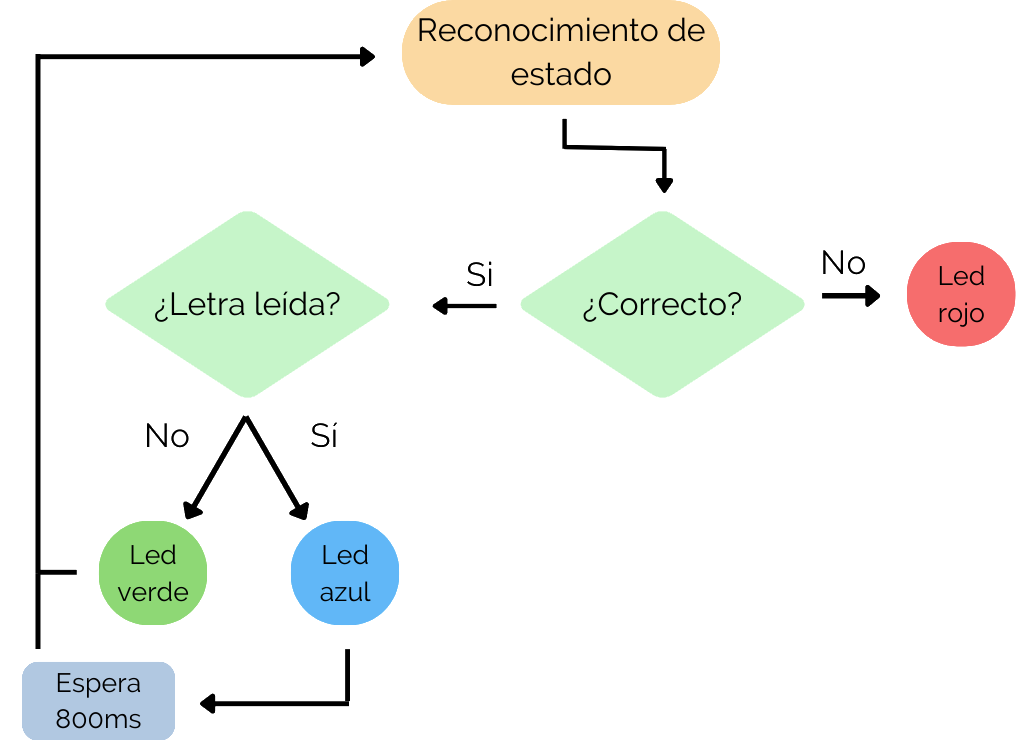
\includegraphics[width=0.8\textwidth]{capturas/diagramaLeds.png}\\[-0,20cm]
    \caption{Diagrama de funcionamiento de los leds}
\end{figure}\\
En estado idle el led
encendido será el verde y en estado de detección de letra, será azul(quedará en este estado
durante 800ms, tiempo durante el que no se detectará nada, para que el usuario pueda
reposicionar su postura para volver a escribir otra letra); en caso de que la \textbf{IMU}
no esté disponible, se encenderá el led rojo.\newline
Para notificar solo una vez la conexión a un dispositivo,
se crea una pequeña estructura para consultar el estado de conexión de la iteración
anterior(\textit{last\_connection}). De esta forma es posible mantener consistencia
en la conexión pese a estar dentro de un bucle.\newline
En cuanto al registro de movimiento, se han utilizado algunas de las funciones
del trabajo de \textit{Pete Warden} y su \textit{magic\_wand}\textsuperscript{\cite{petewardenmw}}
a modo de librería para mi propio proyecto y así aligerar el desarrollo de
la recolección de trazos y su rasterización.\newline
Durante este proceso, se hará uso del giroscopio para determinar los cambios del trazo y el acelerometro
para pequeños ajustes sobre los resultados obtenidos con el giroscopio, por ejemplo
cálculos de gravedad y parámetros de velocidad del cambio de trayectoria del trazo.
Gracias a contar con las funciones antes citadas, tomar los valores de los sensores
es tan fácil como llamar a la función \textit{ReadAccelerometerAndGyroscope}.
Con los valores leídos, se hace un pequeño arreglo de estimación de desvío del giroscopio
y se envían los valores leídos como característica del servicio para \textit{Data Collector}.\newline
Y con el trazo completamente construido y corregido, rasterizamos el movimiento para
obtener la imagen que pasará por el modelo.\newline
Ya está todo listo para dar comienzo con el procesamiento en el modelo. Para llamar a la ejecución,
se invoca el interprete, que arrojará los resultados en un puntero anteriormente definido.
Este puntero de salida, contiene los datos asociados al tensor, es decir, el producto
de que el trazo rasterizado haya pasado por la red neuronal. En nuestro caso, lo que
se obtiene de la red neuronal, es una valoración de ajuste de afinidad del trazo rasterizado
a lo que el modelo ha sido entrenado para reconocer como letras(nuestros \textit{labels}).\newline
Sintetizando, lo que se recibe es una valoración de semejanza a cada letra(codificada como
un índice).\newline
Por tanto, lo que resta es trivial, solo tenemos que obtener el \textit{label} con mayor valoración.
Y como consecuencia, la letra que el modelo ha estimado más posible respecto a su entrenamiento.\newline
Obtenida la letra, es enviada al puerto serie, para cuando se trabaje con conexión física;
y se introduce en la característica de transferencia(\textit{tx}) para el servicio BLE.\newline
Como comprobación concluyente, se verifica si la característica de lectura(\textit{rx}) ha sido
escrita por el programa de usuario, suponiendo esto una señal de que ya ha sido leída la letra
actual en \textit{tx} y como consecuencia, haciendo que se restaure su valor a uno por defecto;
ya que de no hacerlo, la letra permanecería inmutable en la característica y el programa
de usuario leería las mismas letras reiteradamente hasta escribir otras.
Esto se debe a que el las \textit{características} en \textit{BLE} funcionan con valores
constantes hasta que se modifique el estado actual.
